\documentclass{article}

% Things for drawing factor graphs nicely
\usepackage{tikz}
% \usetikzlibrary{shapes.geometric, arrows, fit}
\usetikzlibrary{positioning, shapes.arrows, arrows.meta}
\definecolor{blue}{RGB}{0,128,255}
\definecolor{green}{RGB}{15,180,0}
\definecolor{yellow}{RGB}{255,226,0}
\tikzstyle{hidden}=[circle, minimum size = .9cm, draw=black, thick]
\tikzstyle{factor}=[rectangle, draw=black,fill=black,text=white]
\tikzstyle{dyn}=[rectangle, draw=green,fill=green]
\tikzstyle{prior}=[rectangle, draw=black,fill=yellow,text=black]

\begin{document}
\begin{figure}[htbp!]
    \begin{tabular}{@{}c@{}}
        \resizebox{\textwidth}{!}{
        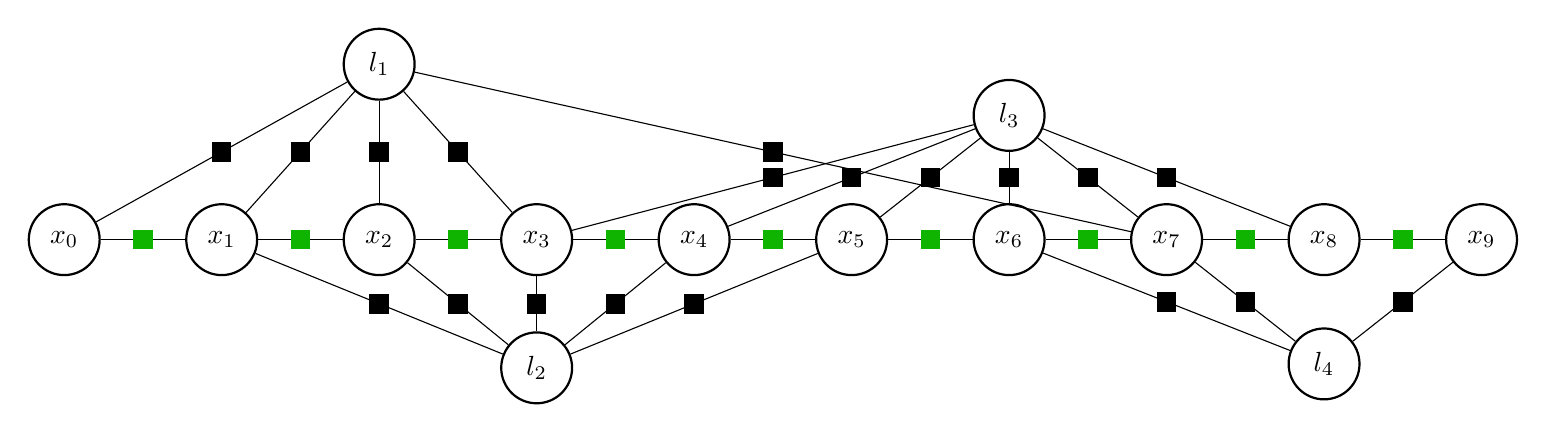
\begin{tikzpicture}
            %Visual odometery type graph with dynamics skipping some hidden factors
            \node[hidden](x0){$x_0$};
            \foreach \n in {1,...,9}{
                \pgfmathtruncatemacro\nmm{\n -1}
                \node[factor, right of = x\nmm, green](d\nmm){};
                \node[hidden,right of = d\nmm](x\n){$x_\n$};
                \draw (x\nmm) to (d\nmm);
                \draw (d\nmm) to (x\n);
            }
            % landmark 1
            \node[hidden, above = 1.3cm of x2](l1){$l_1$};
            \foreach \n in {0,1,2,3,7}{
                \draw (x\n) -- (l1) node[factor, midway] {} ;
            }
            % landmark 2
            \node[hidden, below = .7cm of x3](l2){$l_2$};
            \foreach \n in {1,2,3,4,5}{
                \draw (x\n) -- (l2) node[factor, midway] {} ;
            }
            % landmark 3
            \node[hidden, above = .65cm of x6](l3){$l_3$};
            \foreach \n in {3,4,5,6,7,8}{
                \draw (x\n) -- (l3) node[factor, midway] {} ;
            }
            % landmark 4
            \node[hidden, below = .65cm of x8](l4){$l_4$};
            \foreach \n in {6,7,9}{
                \draw (x\n) -- (l4) node[factor, midway] {} ;
            }
        \end{tikzpicture}
        } \\
        (a) Graph representing typical SLAM problem \\[1em]

        \resizebox{\textwidth}{!}{
        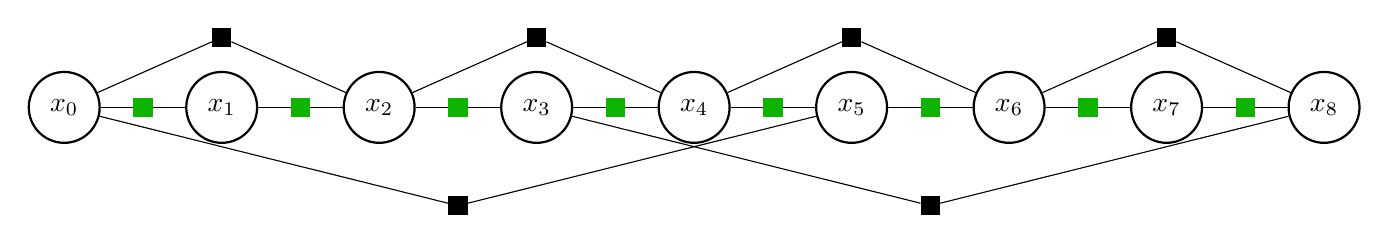
\begin{tikzpicture}
            %Visual odometery type graph with dynamics skipping some hidden factors
            \node[hidden](x0){$x_0$};
            \foreach \n in {1,...,8}{
                \pgfmathtruncatemacro\nmm{\n -1}
                \node[factor, right of = x\nmm, green](d\nmm){};
                \node[hidden,right of = d\nmm](x\n){$x_\n$};
                \draw (x\nmm) to (d\nmm);
                \draw (d\nmm) to (x\n);
            }
            \foreach \n in {0,2,...,6}{
                \pgfmathtruncatemacro\nptwo{\n +2}
                \pgfmathtruncatemacro\npp{\n +1}
                \node[factor, above = .3cm of x\npp](vo\n-2){};
                \draw(x\n) to (vo\n-2);
                \draw(vo\n-2) to (x\nptwo);
            }
            \foreach \n in {0,3}{
                \pgfmathtruncatemacro\npfive{\n +5}
                \pgfmathtruncatemacro\nptwo{\n +2}
                \node[factor, below = 1cm of d\nptwo](vo\n-5){};
                \draw(x\n) to (vo\n-5);
                \draw(vo\n-5) to (x\npfive);
            }
            
        \end{tikzpicture}
        } \\
        (b) Graph with relative measurements between different time steps \\[1em]
        
        % Graph with multiple dynamics
        \resizebox{\textwidth}{!}{
        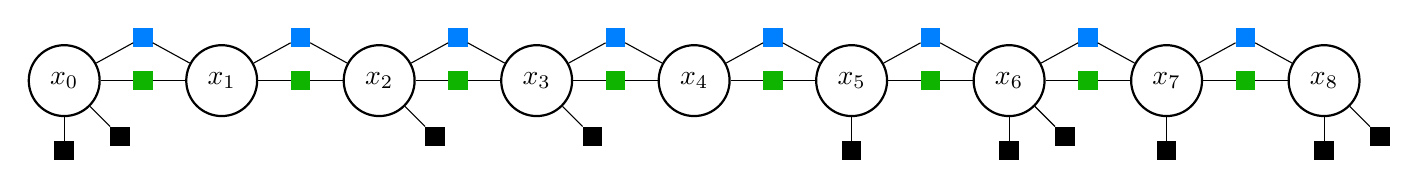
\begin{tikzpicture}
            %Visual odometery type graph with dynamics skipping some hidden factors
            \node[hidden](x0){$x_0$};
            \node[factor, below =.3cm of x0](m0){};
            \draw(x0) to (m0);
            \foreach \n in {1,...,8}{
                \pgfmathtruncatemacro\nmm{\n -1}
                \node[factor, right of = x\nmm,green](d\nmm){};
                \node[hidden,right of = d\nmm](x\n){$x_\n$};
                \node[factor, above = .3cm of d\nmm, blue](d2-\nmm){};
                \ifnum \n>4 \relax
                    \node[factor, below = .3cm of x\n](m\n){};
                    \draw (x\n) to (m\n);
                \fi
                \draw (x\nmm) to (d\nmm);
                \draw (d\nmm) to (x\n);
                \draw (x\nmm) to (d2-\nmm);
                \draw (d2-\nmm) to (x\n);
            }
            \foreach \n in {0,2,3,6,8}{
                \node[factor, below right of = x\n](f2-\n){};
                \draw(x\n) to (f2-\n);
            }
        \end{tikzpicture}
        } \\
        (c) Graph with different dynamics models between time steps and non-periodic measurements \\[1em]
        
        % Graph with multiple dynamics and discrete selector (with prior)
        \resizebox{\textwidth}{!}{
        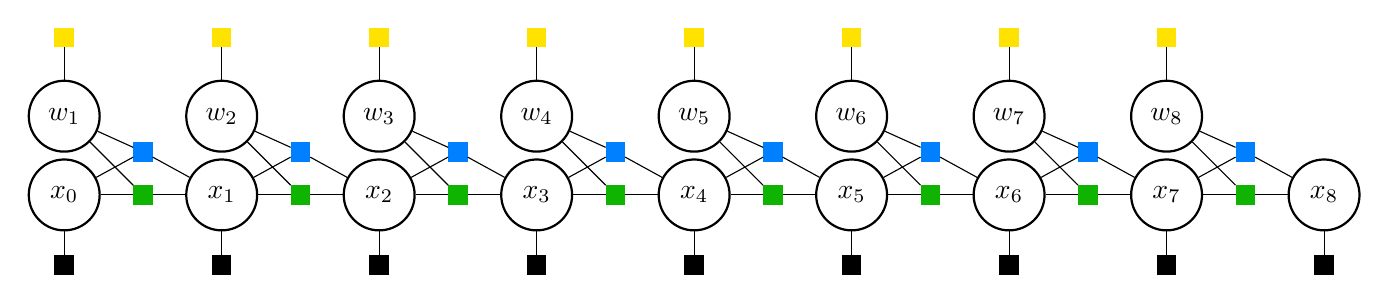
\begin{tikzpicture}
            %Visual odometery type graph with dynamics skipping some hidden factors
            \node[hidden](x0){$x_0$};
            \node[factor, below =.3cm of x0](m0){};
            \draw(x0) to (m0);
            \foreach \n in {1,...,8}{
                \pgfmathtruncatemacro\nmm{\n -1}
                \node[factor, right of = x\nmm,green](d\nmm){};
                \node[hidden,right of = d\nmm](x\n){$x_\n$};
                \node[factor, above = .3cm of d\nmm, blue](d2-\nmm){};
                \node[factor, below = .3cm of x\n](m\n){};
                \node[hidden,above of = x\nmm](ds\nmm){$w_\n$};
                \node[factor,above of = ds\nmm, yellow](pds\nmm){};
                \draw (pds\nmm) to (ds\nmm);
                \draw (ds\nmm) to (d2-\nmm);
                \draw (ds\nmm) to (d\nmm);
                \draw (x\n) to (m\n);
                \draw (x\nmm) to (d\nmm);
                \draw (d\nmm) to (x\n);
                \draw (x\nmm) to (d2-\nmm);
                \draw (d2-\nmm) to (x\n);
            }
        \end{tikzpicture}
        } \\
        (d) Graph with additional hidden variables nodes for selecting weighting of the dynamics models \\[1em]
        
        \resizebox{.8\textwidth}{!}{
        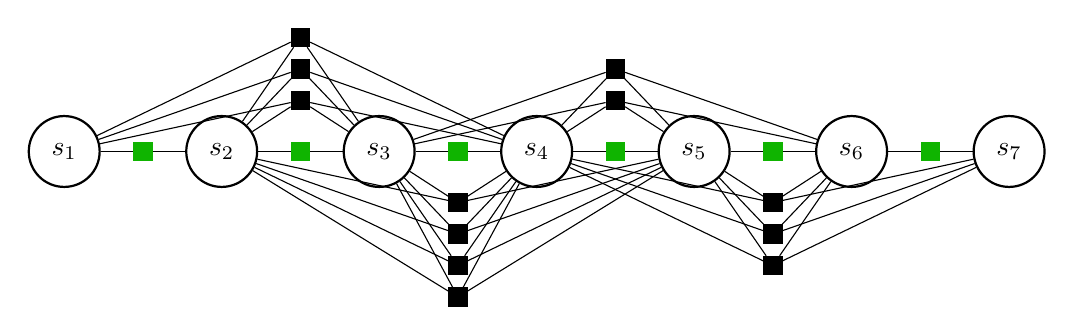
\begin{tikzpicture}
            %Visual odometery type graph with dynamics skipping some hidden factors
            \node[hidden](x1){$s_1$};
            \foreach \n in {2,...,7}{
                \pgfmathtruncatemacro\nmm{\n -1}
                \node[factor, right of = x\nmm, green](d\nmm){};
                \node[hidden,right of = d\nmm](x\n){$s_\n$};
                \draw (x\nmm) to (d\nmm);
                \draw (d\nmm) to (x\n);
            }
            %Nodes in first time step
            \foreach \n in {1,...,3}{
                \pgfmathsetmacro\offset{\n*.4}
                \node[factor, above = \offset cm of d2](event1-\n){};
                \draw(x1) to (event1-\n);
                \draw(x2) to (event1-\n);
                \draw(x3) to (event1-\n);
                \draw(x4) to (event1-\n);
            }

            %Nodes in second time step
            \foreach \n in {1,...,4}{
                \pgfmathsetmacro\offset{\n*.4}
                \node[factor, below = \offset cm of d3](event1-\n){};
                \draw(x2) to (event1-\n);
                \draw(x3) to (event1-\n);
                \draw(x4) to (event1-\n);
                \draw(x5) to (event1-\n);
            }

            %Nodes in third time step
            \foreach \n in {1,...,2}{
                \pgfmathsetmacro\offset{\n*.4}
                \node[factor, above = \offset cm of d4](event1-\n){};
                \draw(x3) to (event1-\n);
                \draw(x4) to (event1-\n);
                \draw(x5) to (event1-\n);
                \draw(x6) to (event1-\n);
            }

            %Nodes in second time step
            \foreach \n in {1,...,3}{
                \pgfmathsetmacro\offset{\n*.4}
                \node[factor, below = \offset cm of d5](event1-\n){};
                \draw(x4) to (event1-\n);
                \draw(x5) to (event1-\n);
                \draw(x6) to (event1-\n);
                \draw(x7) to (event1-\n);
            }
        \end{tikzpicture}
        } \\
        (e) Graph for use with very fine-scaled time-based sensors
    \end{tabular}
    \caption{Examples of different graphs that can be solved using factor graphs that are not standard Kalman filter type graphs.}
    \label{fig:diffGraphs}
\end{figure}

\end{document}